
        \documentclass[spanish, 11pt]{exam}

        %These tell TeX which packages to use.
        \usepackage{array,epsfig}
        \usepackage{amsmath, textcomp}
        \usepackage{amsfonts}
        \usepackage{amssymb}
        \usepackage{amsxtra}
        \usepackage{amsthm}
        \usepackage{mathrsfs}
        \usepackage{color}
        \usepackage{multicol, xparse}
        \usepackage{verbatim}


        \usepackage[utf8]{inputenc}
        \usepackage[spanish]{babel}
        \usepackage{eurosym}

        \usepackage{graphicx}
        \graphicspath{{../img/}}



        \printanswers
        \nopointsinmargin
        \pointformat{}

        %Pagination stuff.
        %\setlength{\topmargin}{-.3 in}
        %\setlength{\oddsidemargin}{0in}
        %\setlength{\evensidemargin}{0in}
        %\setlength{\textheight}{9.in}
        %\setlength{\textwidth}{6.5in}
        %\pagestyle{empty}

        \let\multicolmulticols\multicols
        \let\endmulticolmulticols\endmulticols
        \RenewDocumentEnvironment{multicols}{mO{}}
         {%
          \ifnum#1=1
            #2%
          \else % More than 1 column
            \multicolmulticols{#1}[#2]
          \fi
         }
         {%
          \ifnum#1=1
          \else % More than 1 column
            \endmulticolmulticols
          \fi
         }
        \renewcommand{\solutiontitle}{\noindent\textbf{Sol:}\enspace}

        \newcommand{\samedir}{\mathbin{\!/\mkern-5mu/\!}}

        \newcommand{\class}{1º Bachillerato}
        \newcommand{\examdate}{\today}

        \newcommand{\tipo}{A}


        \newcommand{\timelimit}{50 minutos}



        \pagestyle{head}
        \firstpageheader{
\includegraphics[width=0.2\columnwidth]{header_left}}{\textbf{Departamento de Matemáticas\linebreak \class}\linebreak \examnum}{
\includegraphics[width=0.1\columnwidth]{header_right}}
        \runningheader{\class}{\examnum}{Página \thepage\ of \numpages}
        \runningheadrule

        \newcommand{\examnum}{Autoevaluación 2 ev1}
        \begin{document}
        \begin{questions}
        \question p015e09 - Efectúa simplificando el resultado si es posible:
        \begin{multicols}{2} 
        \begin{parts} \part[1]  $ \frac{\frac{x^2+2x+1}{x - 3}}{\frac{x+1}{x^2 -9 }} $  \begin{solution}  $ x^{2} + 4 x + 3 $  \end{solution} \part[1]  $ \frac{3x^2+1}{x^2+x}  - \frac{2x}{x+1} $  \begin{solution}  $ \frac{x^{2} + 1}{x^{2} + x} $  \end{solution} \part[1]  $ \frac{\frac{x^2-2x+1}{x + 3}}{\frac{x-1}{x^2 -9 }} $  \begin{solution}  $ x^{2} - 4 x + 3 $  \end{solution} \part[1]  $ \frac{3x^2+1}{x^2+x}  - \frac{2x}{x+1} $  \begin{solution}  $ \frac{x^{2} + 1}{x^{2} + x} $  \end{solution} \part[1]  $ \frac{1}{x^2-x} + \frac{2x-1}{x-1} - \frac{3x-1}{x} $  \begin{solution}  $ - \frac{x - 3}{x - 1} $  \end{solution} \part[1]  $ \frac{x}{{1 + \frac{1}{{1 + \frac{1}{x}}}}} $  \begin{solution}  $ \frac{x^{2} + x}{2 x + 1} $  \end{solution} \part[1]  $ \frac{{\frac{x}{{x - 2}} - \frac{x}{{x + 2}}}}{{1 - \frac{4}{{{x^2} - 4}}}} $  \begin{solution}  $ \frac{4 x}{x^{2} - 8} $  \end{solution} \part[1]  $ \frac{1}{{\frac{{x + 1}}{{x - 1}} - \frac{{x - 1}}{{x + 1}}}} $  \begin{solution}  $ \frac{x^{2} - 1}{4 x} $  \end{solution} \part[1]  $ ( {{x^3} + x} )\cdot( {1 - \frac{{2x}}{{2x + \frac{2}{x}}}}) $  \begin{solution}  $ x $  \end{solution} \part[1]  $ ( {\frac{1}{x} - \frac{1}{{x + 1}}})( {x - \frac{{x + 1}}{{x - 1}}}) $  \begin{solution}  $ \frac{x^{2} - 2 x - 1}{x^{3} - x} $  \end{solution} \part[1]  $ \frac{1}{x}( {\frac{2}{x} - \frac{3x}{{x + 1}}} ) - \frac{{x}}{x-1}( {3 - \frac{4}{{x + 1}}} ) $  \begin{solution}  $ - \frac{3 x^{4} + 2 x^{3} - 5 x^{2} + 2}{x^{4} - x^{2}} $  \end{solution} \part[1]  $ \frac{{\frac{{x - 1}}{{x + 2}} - \frac{{x + 2}}{{x - 1}}}}{{1 - \frac{1}{{x - 1}}}} $  \begin{solution}  $ - \frac{6 x + 3}{x^{2} - 4} $  \end{solution}
        \end{parts}
        \end{multicols}
        \question p020e02-e16 - Resuelve mediante expresiones algebraicas:
        \begin{multicols}{1} 
        \begin{parts} \part[1] En un corral hay conejos y gallinas, en total 50 cabezas y 134 patas. 
    ¿Cuántos animales hay de cada clase?  \begin{solution}  $ \left\{\begin{matrix}50=x+y\\ 134=4x+2y\\ \end{matrix}\right.  \rightarrow  \\\left[\begin{matrix}1 & 1 & 50\\0 & 2 & 34\end{matrix}\right] \rightarrow  \left \{ x : 17, \quad y : 33\right \} $  \end{solution} \part[1] Se tienen 140 euros, en 20 billetes, unos de 5 euros y de 10 los restantes. 
    ¿Cuántos billetes hay de cada clase?  \begin{solution}  $ \left\{\begin{matrix}140=5x+10y\\ 20=x+y\\ \end{matrix}\right.  \rightarrow  \\\left[\begin{matrix}10 & 5 & 140\\0 & \frac{1}{2} & 6\end{matrix}\right] \rightarrow  \left \{ x : 12, \quad y : 8\right \} $  \end{solution} \part[1] Un librero vendió 84 libros, unos a 45 euros y otros a 36 y obtuvo de la venta 3.105 euros. ¿Cuántos vendió de
cada clase?  \begin{solution}  $ \left\{\begin{matrix}3105=45x+36y\\ 84=x+y\\ \end{matrix}\right.  \rightarrow  \\\left[\begin{matrix}36 & 45 & 3105\\0 & - \frac{1}{4} & - \frac{9}{4}\end{matrix}\right] \rightarrow  \left \{ x : 9, \quad y : 75\right \} $  \end{solution} \part[1] En una clase los 2/3 del número de alumnas es igual a los 5/7 del número de alumnos. Si el número de
alumnas aumenta en 26, entonces es igual al doble del número de alumnos. ¿Cuántos alumnos y alumnas
tiene la clase?  \begin{solution}  $ \left\{\begin{matrix}\frac{2x}{3}=\frac{5y}{7}\\ x+26=2y\\ \end{matrix}\right.  \rightarrow  \\\left[\begin{matrix}\frac{2}{3} & - \frac{5}{7} & 0\\0 & \frac{13}{14} & 26\end{matrix}\right] \rightarrow  \left \{ x : 30, \quad y : 28\right \} $  \end{solution}
        \end{parts}
        \end{multicols}
        \question p021e23 - Resuelve los sistemas:
        \begin{multicols}{2} 
        \begin{parts} \part[1]  $ \left\{\begin{matrix}2x-y+2z=1\\ x+y-z = 3\\ 3x+2y+z =  5\\ \end{matrix}\right. $  \begin{solution}  $ \left[\begin{matrix}2 & 2 & -1 & 1\\0 & 2 & \frac{1}{2} & \frac{7}{2}\\0 & 0 & 2 & 1\end{matrix}\right] \rightarrow  \\ \left \{ x : \frac{13}{8}, \quad y : \frac{1}{2}, \quad z : - \frac{7}{8}\right \} $  \end{solution} \part[1]  $ \left\{\begin{matrix}x - y + z = 1\\ 2x + y - 2z = 2\\ x+2y-3z = 1\\ \end{matrix}\right. $  \begin{solution}  $ \left[\begin{matrix}1 & 1 & -1 & 1\\0 & 4 & -1 & 4\\0 & 0 & 0 & 0\end{matrix}\right] \rightarrow  \\ \left \{ x : \frac{z}{3} + 1, \quad y : \frac{4 z}{3}\right \} $  \end{solution} \part[1]  $ \left\{\begin{matrix}x+y+z=1\\ x + 2y - z = 2\\ 2x +3y = 4\\ \end{matrix}\right. $  \begin{solution}  $ \left[\begin{matrix}1 & 1 & 1 & 1\\0 & 2 & 3 & 3\\0 & 0 & 0 & 1\end{matrix}\right] \rightarrow  \\ \left [ \right ] $  \end{solution} \part[1]  $ \left\{\begin{matrix}x+y+z=1\\ x + 2y - z = 2\\ 2x +3y = 3\\ \end{matrix}\right. $  \begin{solution}  $ \left[\begin{matrix}1 & 1 & 1 & 1\\0 & 2 & 3 & 3\\0 & 0 & 0 & 0\end{matrix}\right] \rightarrow  \\ \left \{ x : - 3 z, \quad y : 2 z + 1\right \} $  \end{solution} \part[1]  $ \left\{\begin{matrix}\frac{x}{2} + \frac{y}{3} + z = -\frac{1}{2}\\ x - \frac{y}{2} + \frac{z}{3} = -1\\  \frac{x}{3} - y - \frac{z}{2} = -\frac{1}{6}\\ \end{matrix}\right. $  \begin{solution}  $ \left[\begin{matrix}1 & \frac{1}{2} & \frac{1}{3} & - \frac{1}{2}\\0 & \frac{5}{6} & - \frac{11}{18} & - \frac{5}{6}\\0 & 0 & - \frac{73}{180} & \frac{1}{6}\end{matrix}\right] \rightarrow  \\ \left \{ x : - \frac{95}{73}, \quad y : - \frac{30}{73}, \quad z : \frac{21}{73}\right \} $  \end{solution} \part[1]  $ \left\{\begin{matrix}\frac{x}{2} + \frac{y}{3} + \frac{z}{3} = -2\\ \frac{x}{3} - \frac{y}{2} + \frac{z}{3} = 2\\ \frac{x}{6} + \frac{y}{2} + \frac{z}{2} = 1\\ \end{matrix}\right. $  \begin{solution}  $ \left[\begin{matrix}\frac{1}{3} & \frac{1}{2} & \frac{1}{3} & -2\\0 & - \frac{1}{6} & - \frac{5}{6} & 4\\0 & 0 & \frac{35}{12} & -10\end{matrix}\right] \rightarrow  \\ \left \{ x : - \frac{48}{7}, \quad y : - \frac{24}{7}, \quad z : \frac{54}{7}\right \} $  \end{solution} \part[1]  $ \left\{\begin{matrix}x - y + z = 5\\ \frac{{x - 1}}{2} + \frac{y}{3} = 1\\ \frac{{2x + y}}{2} - \frac{{3z + y}}{3} = 4\\ \end{matrix}\right. $  \begin{solution}  $ \left[\begin{matrix}1 & 1 & -1 & 5\\0 & \frac{1}{2} & \frac{1}{3} & \frac{3}{2}\\0 & 0 & - \frac{13}{6} & 3\end{matrix}\right] \rightarrow  \\ \left \{ x : \frac{51}{13}, \quad y : - \frac{18}{13}, \quad z : - \frac{4}{13}\right \} $  \end{solution}
        \end{parts}
        \end{multicols}
        \question p026e07 - Resuelve los siguientes sistemas de inecuaciones:
        \begin{multicols}{2} 
        \begin{parts} \part[1]  $ \left\{\begin{matrix}\frac{{x - 1}}{2} - \frac{{x + 3}}{3} \leq x\\ \frac{{4x - 2}}{4} - \frac{{x - 1}}{3} \geq x\end{matrix}\right. $  \begin{solution}  $ \left[- \frac{9}{5}, - \frac{1}{2}\right] $  \end{solution} \part[1]  $ \left\{\begin{matrix}{( {x - 1} )^2} - {( {x + 3} )^2} \leq 0\\x - 3( {x - 1}^2 ) \leq 3 \end{matrix}\right. $  \begin{solution}  $ \left[-1, \infty\right) $  \end{solution} \part[1]  $ \left\{\begin{matrix}\frac{{3( {2 - x} )}}{2} - x < \frac{{16}}{3} - \frac{{x + 1}}{5} \\\frac{{x + 4}}{3} - \frac{{x - 5}}{6} > 3 - \frac{{2x - 3}}{{18}}\end{matrix}\right. $  \begin{solution}  $ \left(\frac{18}{5}, \infty\right) $  \end{solution}
        \end{parts}
        \end{multicols}
        \question p026e08 - Resuelve los siguientes sistemas de inecuaciones:
        \begin{multicols}{2} 
        \begin{parts} \part[1]  $ \left\{\begin{matrix}x + y \leq 2 \\ - 2x + y \geq 4\\\end{matrix}\right. $  \begin{solution}   \\ 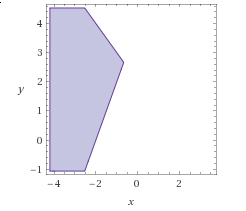
\includegraphics[width=1\columnwidth]{si0}   \end{solution} \part[1]  $ \left\{\begin{matrix}2x - y < 1 \\ - x + 4y \geq  - 5\\\end{matrix}\right. $  \begin{solution}   \\ 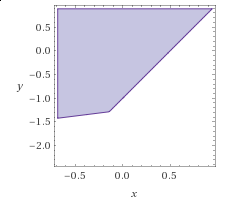
\includegraphics[width=1\columnwidth]{si1}   \end{solution} \part[1]  $ \left\{\begin{matrix}x - 2y > 3\\5x - 3y \leq 15\\\end{matrix}\right. $  \begin{solution}   \\ 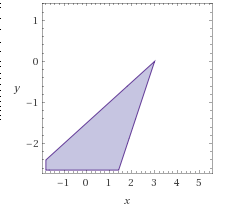
\includegraphics[width=1\columnwidth]{si2}   \end{solution} \part[1]  $ \left\{\begin{matrix}x \geq y \\x + y \geq 4\\x - 2y \leq 8\\\end{matrix}\right. $  \begin{solution}   \\ 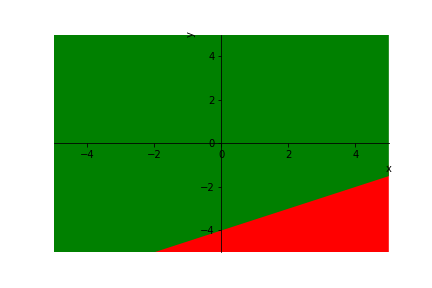
\includegraphics[width=1\columnwidth]{si3}   \end{solution} \part[1]  $ \left\{\begin{matrix}- 2 \leq x\\x \leq 2\\y \geq 4\\x + y - 1 \leq 0\\\end{matrix}\right. $  \begin{solution}   \\ 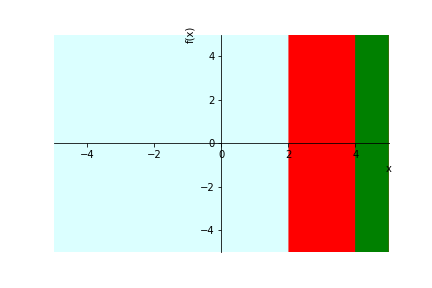
\includegraphics[width=1\columnwidth]{si4}   \end{solution} \part[1]  $ \left\{\begin{matrix}x \geq 0 \\0 \leq y\\y \leq 3\\x - 2y \leq 10\\x + y \geq 10\\\end{matrix}\right. $  \begin{solution}   \\ 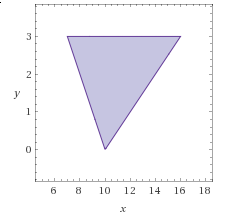
\includegraphics[width=1\columnwidth]{si5}   \end{solution}
        \end{parts}
        \end{multicols}
        
    \end{questions}
    \end{document}
    